\subsection{Linear Functions}
A linear function is a function whose graph is a straight line. Its degree is 1 or 0. It has a constant rate of change.

\subsubsection{Slope}
Slope is a measure of how one quantity changes with respect to another, sometimes called the rate of change. For graphs, it is determined by calculating the change in the y-values over the change in x-values and is denoted by $m$.
$$m=\frac{\Delta y}{\Delta x}=\frac{y_2-y_1}{x_2-x_1}$$
For example, a line with slope $\frac{3}{2}$ will go up 3 units for every 2 units it goes across.\\
- Horizontal lines will always have a slope of 0.\\
- Vertical lines have an undefined slope ($\frac{1}{0}$).\\
- Parallel lines will have the same slope: $m_\parallel=m$.\\
- Perpendicular lines will have a slope that is equal to the negative reciprocal of the other. ${m_\perp=-\dfrac{1}{m}}$

\subsubsection{Equations of Linear Functions}
\begin{itemize}
    \item Slope Intercept Form: $y=mx+b$\\
    where $m$ is the slope and $b$ is the y-intercept. Slope intercept form is ideal for graphing the function and is the most commonly used.
    \item Slope Point Form: $y-y_1=m(x-x_1)$\\
    where $(x_1,y_1)$ is some point on the line. This is useful for when you are given a point and the slope and are asked to find an equation.
    \item General Form: $Ax+By+C=0$\\
    where $A$ must be a whole number and $B$ and $C$ are both integers. This is helpful for finding x and y intercepts.
\end{itemize}
All three forms are interchangeable.\\
\\
\textbf{Solving Linear Equations}\\
Often we are interested in when the line crosses the x-axis. We can find this by setting $y=0$ and solving for $x$.\\
Ex: $y=6x+4$
\begin{align*}
    0=&6x+4\\
    -4=&6x\\
    x=&-\frac{2}{3}
\end{align*}

\subsubsection{Systems of Linear Equations}
A system of linear equations is composed of two linear equations and is often referred to as a linear system.\\
A system will have no solutions if the lines are parallel.\\
A system will have infinite solutions if the lines are identical.\\
Otherwise, the system will have one solution.\\
\\
Solving Graphically:\\
The solution of a linear system can be estimated by graphing both equations. The solution will be where the two lines intersect. This will give a point that satisfies both equations. To verify the solution, you can plug the point back in to the original equations.\\
\centerline{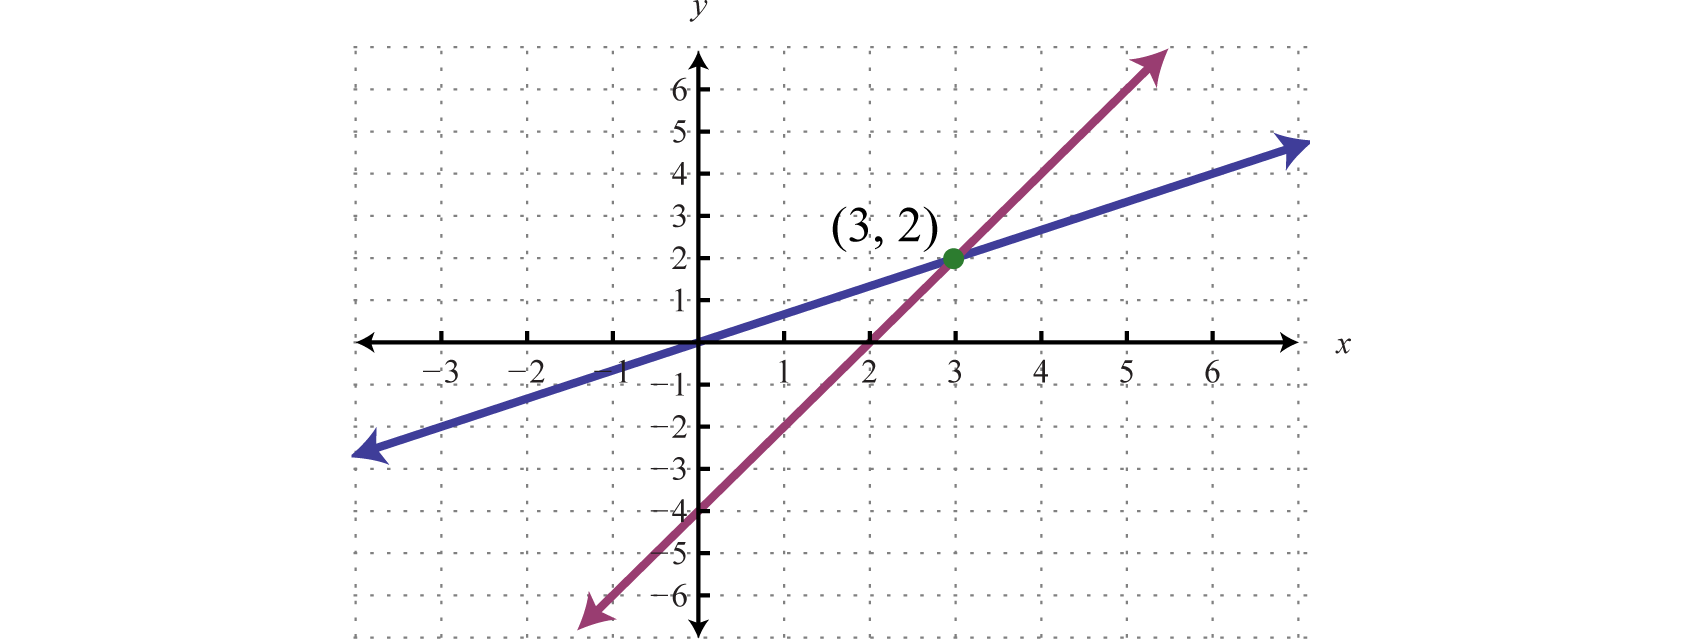
\includegraphics[scale=0.7]{Images/PreCalcPictures/LinearSystemIntersection.png}}
Solving by Elimination\\
Step 1 is to make the value of $x$ or $y$ the same for both equations.\\
Step 2 is to add or subtract the add or subtract the equations to cancel out one of the variables.\\
Step 3 is to solve for the remaining variable.\\
Step 4 is to plug the value back into one of the original equations to solve for the other variable.\\
Ex: $\left\{\begin{matrix} 5x-3y=18\\
4x-6y=18 \end{matrix}\right.$
\begin{align*}
    &\left\{\begin{matrix}
    2(5x-3y=18)\\
    4x-6y=18
    \end{matrix}\right.\\
    &\left\{\begin{matrix}
    10x-6y=36\\
    4x-6y=18
    \end{matrix}\right.\\
    &(10x-6y)-(4x-6y)=36-18\\
    &6x=18\\
    &x=3\\
    &5(3)-3y=18\\
    &15-3y=18\\
    &-3y=3\\
    &y=-1\\
    &\mathrm{Solution}\,\mathrm{is}\,(3,-1)
\end{align*}
Solving by Substitution:\\
Step 1 is to isolate one of the variables in one equation.\\
Step 2 is, in the other equation, replace the variable you isolated for earlier with the equation that it's in terms of.\\
Step 3 is to solve for the remaining variable.\\
Step 4 is to plug the value bck into one of the original equations to solve for the other variable.\\
Ex: $\left\{\begin{matrix} x-3y=12\\
4x+2y=8 \end{matrix}\right.$
\begin{align*}
    & x=3y+12\\
    &4(3y+12)+2y=8\\
    &48+12y+2y=8\\
    &14y=-40\\
    &y=-\frac{20}{7}\\
    &x-3\left(-\frac{20}{7}\right)=12\\
    &x+\frac{60}{7}=\frac{84}{7}\\
    &x=\frac{24}{7}\\
    &\mathrm{Solution}\,\mathrm{is}\,\left(\frac{24}{7},-\frac{20}{7}\right)
\end{align*}

\subsubsection{Linear Inequalities}
Inequalities are in the form of $y\geq f(x)$. It creates a boundary, splitting the Cartesian plane into two or more regions. For $y\geq f(x)$, any part above the function is shaded and for $y\leq f(x)$, any part below the function is shaded. If $\geq$ or $\leq$ are used, the boundary will have a solid line. If $>$ or $<$ are used, the boundary will have dashed line.\\
\centerline{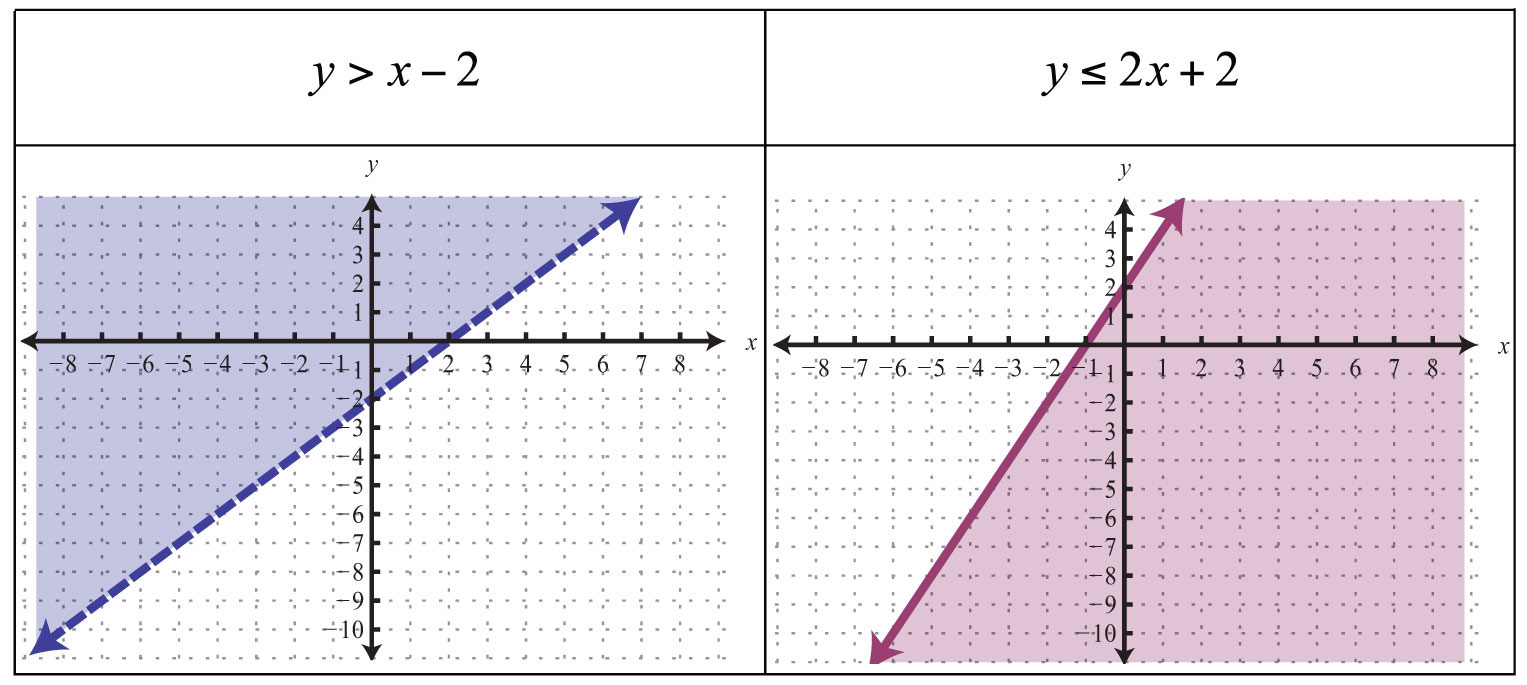
\includegraphics[scale = 0.3]{Images/PreCalcPictures/LinearInequalities.jpg}}